\documentclass{report}
\usepackage[utf8]{inputenc}
\usepackage{amsmath}
\usepackage{amssymb}
\usepackage{graphicx}
\usepackage{pdfpages}
\usepackage{makeidx}
\usepackage[margin=0.75in]{geometry}
\usepackage{parskip}
\usepackage{float}
\usepackage{booktabs}
\usepackage{titlesec}
\usepackage{caption}
\usepackage{subcaption}
\usepackage{hyperref}
\usepackage{enumitem}

%Command to Reference footnotes
\makeatletter
\newcommand\footnoteref[1]{\protected@xdef\@thefnmark{\ref{#1}}\@footnotemark}
\makeatother

%Formating Chapter spacing and linebreak
\titleformat{\chapter}[hang] 
{\normalfont\huge\bfseries}{\chaptertitlename\ \thechapter:}{1em}{}
\titlespacing*{\chapter}{0pt}{0pt}{5pt}

%Removing indent before items on list
%\setlist[itemize]{leftmargin=*}

%Setting space between lines
% \setlength{\baselineskip}{-1.0pt}
\renewcommand{\baselinestretch}{1.0}

%Merging list of tables and figures
\def\table{\def\figurename{Table}\figure}
\let\endtable\endfigure 
\renewcommand\listfigurename{List of Figures and Tables} %Renaming Title of List of Figures

\newcommand{\matr}[1]{\mathbf{#1}}   %Used to indicate a matrix
\newcommand{\vetr}[1]{\overline{#1}} %Used to indicate a Vector

%Capitalising \autoref
\renewcommand*{\chapterautorefname}{Chapter}
\renewcommand*{\subsectionautorefname}{Subsection}
\renewcommand*{\sectionautorefname}{Section}

\hypersetup{
  %hidelinks    = false, %Remove color box
  frenchlinks  = false, %Small caps for hyperlinks
  colorlinks   = true, %Colours links instead of boxes
  urlcolor     = blue, %Colour for external hyperlinks
  linkcolor    = black, %Colour of internal links
  citecolor   = black   %Colour of citations
}

\begin{document}

\pagenumbering{roman}                %Start roman numbering

\begin{titlepage}
	\centering
	\vspace{0.25cm}
	{\scshape\Large MTHM036 - CA3\par}
	\vspace{0.5cm}
	%{\huge\bfseries Marine heat waves under climate change and their effects on the health of phytoplankton \par}
	{\huge\bfseries Marine heat waves and their effects on the health of phytoplankton \par}
	{\Large Candidate Number: 142408}
	\vspace{0.2cm}
	\flushleft
	Supervised by	Dr.~John \textsc{Bruun} \hfill	{\large \today\par}
    \par
    \centering
	%{\large \textbf{Abstract}}
	\par
    
    %Insert some cool abstract that makes our examiner go, "hmm that's a pretty good abstract".

    \vfill
    %Here are the M\textsc{atlab} files to reproduce our findings: \attachfile{Matlab Files} 
\end{titlepage}          %Title Page

\begingroup
\let\clearpage\relax                 %Disable page break from \listoffigures
\renewcommand{\baselinestretch}{1.0} %Set spacing for TOC

\tableofcontents %Table of contents

\listoffigures

\endgroup %Return

\chapter{Introduction}\pagenumbering{arabic} %Switch to normal numbers

Phytoplankton are photosynthesizing components of the plankton community that inhabit the upper light lit layers of water in almost all oceans and bodies of fresh water. Phytoplankton obtain energy from the Sun through the process, photosynthesis. It is estimated that phytoplankton account for around half of all photosynthetic activity on Earth, \cite{halfO2} yet only account for 1\% of Earth's biomass. \cite{bidle2004cell} 
\\\\
As well as providing half of our atmospheres oxygen, phytoplankton remove large amounts of carbon dioxide from our atmosphere. Through photosynthesis, phytoplankton turn carbon dioxide from our atmosphere into carbonates. Once this carbon is fixed into soft or hard tissue, the organisms either stay in the upper light lit regions to again be used in photosynthesis or once they die, begin to sink to the bottom of the ocean floor. The fixed carbon is then either decomposed by bacteria on the way down or once on the sea floor is remineralized to be used again in primary production. The particles that escape these processes entirely are sequestered at the bottom of the ocean in the ground sediment and may remain there for millions of years. It is this sequestered carbon that is responsible for lowering atmospheric carbon dioxide.
\\\\
It is these important characteristics that give motivation to study the health of phytoplankton and more importantly to understand what can be done to ensure longevity of this vital species. 

\section{Marine Heat Waves and their Impacts}

\begin{quote}
    An extreme event is an event that is rare at a particular place and time of year. Definitions of 'rare' vary, but an extreme event would normally be as rare as or rarer than the 10th or 90th percentile of a probability density function estimated from observations. \hfill\cite[p.~6-8]{IPCC2019}
\end{quote}

Sea temperatures recorded to be extreme for their respective location for a period of five or more consecutive days are so-called marine heat waves (MHWs). Sucessive heatwaves with gaps of two days or less are considered part of the same event. \cite{MWHdef} Marine heatwaves and their effects on natural, physical and socio-economic systems have been well documented in all ocean basins over the last two decades. A notable example is the Northeast Pacific 2013-2015 MWH where extremely high temperatures were linked to the presence of elevated levels of a natural toxin domoic acid (DA) in razor clams \cite{toxinheat}. 
\\\\
Domoic acid is a kainic acid-type neurotoxin that is produced by harmful phytoplankton species. After a large-scale algal bloom in late 2015 levels of DA along the west coast of North America were deemed above safe thresholds. This in turn lead to the closure of recreational razor clam harvest and Dungeness crab fisheries in a variety of locations along the west coast of North America. "Fisheries of the United States 2015" report showed a decreased value of Dungeness crab fished of almost a \$100 million compared to the previous year. \cite{2015Cost} In addition to negative economic impacts, toxic events can lead to the mass death of marine mammals and can pose potential public health issues for humans. Human consumption of shellfish with high levels of DA can cause a neurological disorder called domoic acid poisoning. 

\section{Changes to Marine Heat Waves under Climate Change}
When talking about certainty, we will use the following terms to express the assessed likelihood of an outcome or a result: Virtually certain 99-100\% probability, Very likely 90-100\%, Likely 66-100\%, About as likely as not 33-66\%, Unlikely 0-33\%, Very unlikely 0-10\% and Exceptionally unlikely 0-1\%
\\\\
The International Governmental Panel on Climate Change (IPCC) WGI AR5 report concluded that it is \textit{virtually} certain that the global ocean temperature in the upper few hundred metres has increased from 1971-2010 \cite{AR5}, and is projected to further increase during the twenty-first century. \cite{collins2013long} Concurrent with the long-term increase in the upper ocean temperatures, MHWs have become more frequent, extensive and intense. \cite{1,2,3}
\\\\
Analysis of satellite daily sea surface temperature data from 1982-2016 shows that the number of MHW days above the 99th percentile, between 1982 and 2016 has doubled globally from around 2.5 to 5 heatwave-days per year \cite{1,2}. During the same period the maximum intensity of MHWs has increased by $0.3^\circ$C and the spatial extent by 66\%. \cite{1} The observed trend towards more frequent, extensive and intense MHWs, defined to a fixed baseline period, is \textit{very likely} due to anthropogenic increase in mean ocean temperatures. \cite{1,2,3} As climate models project a long-term increase in ocean temperatures over the 21st century \cite{collins2013long} a further increase in the probability of of MHWs under continued global warming can be expected. \cite{IPCC2019}
\\\\

{\let\clearpage\relax \chapter{Data and methods of analysis}}

In this chapter will discuss the methods we will be using to analysis our data and the sources of the data we will be using. To handle the computation of analysing our data we will be using two popular numerical computing programs, \textsc{MATLAB} and RStudio. The main appeal to using computing software, is firstly the speed and more importantly the ease of repeating the same calculations at different locations.

\section{Data used}

To analysis marine heat waves and their effects on the health of phytoplankton we first needed a set of data that measured the sea surface temperature (SST) across a spatial grid. We then needed a data set containing chlorophyll concentration across a spatial grid, this data is what we will use to monitor the health of phytoplankton, explained in greater detail in \autoref{subsec:chl phyt}

\subsection{Chlorophyll Concentration Data}

To analysis the health of phytoplankton, we use Ocean Colour Climate Change Initiative (OC\_CCI) \cite{ESA} data by the European Space Agency, which consists of globally merged satellite data with associated per-pixel uncertainty information. These satellites are MERIS, Aqua-MODIS, SeaWiFS and VIIRS; on board these satellites are various sensors that measure the characteristics of light coming from the Earth's surface.

Samples of ocean water are taken and their concentrations of phytoplankton and chlorophyll are analyzed, these measurements will then be correlated with the measurements taken from the satellite light readings. Algorithms are then constructed that aim to produce accurate readings of chlorophyll concentration based solely of data obtained from satellites. These algorithms can then be used to produce readings of chlorophyll concentration data over large areas of the Earth.

\subsubsection{Chlorophyll Concentration as an Indicator for Phytoplankton Health}\label{subsec:chl phyt}

Chlorophyll is the material that allows plant cells to convert sunlight into energy, thus enabling them to grow. Since phytoplankton rely on photosynthesis to produce energy, this green substance is a good indicator of overall plant health. By measuring chlorophyll concentration, we can determine the health and growth of phytoplankton.

\subsection{Sea Surface Temperature Data}

Similarly to the chlorophyll concentration data, satellites are able to measure the SST using on board sensors that measure the characteristics of electromagnetic radiation being emitted from the Earth's oceans. The amplitude of these measured wavelengths vary with the temperature of the ocean and therefore can be used to measure temperature.
\\\\
Spatial sea surface temperature data will allow us to identify marine heat waves and also allow us to build correlation models between SST and health of phytoplankton. We will be using the NOAA Optimum Interpolation Sea Surface Temperature by National Centers for Environmental Prediction (NCEP) institution. This data consists of of weekly mean temperatures compututed using a combination of in situ, satellite SST's plus SST's simulated by sea-ice cover. The satelitte data is adjusted for biases using the method of Reynolds \cite{reynolds1988real} and Reynolds and Marsico \cite{1993reynolds}.

\section{Methods of Analysis}

The purpose of data analysis is to extract useful information from our data by making predictions, establishing relationships and correlations and deepen our understanding of the involved mechanisms in our system. In this section will we introduce and briefly explain the method, it's purpose and it's reliability.

\subsection{Auto-regressive Integrated Moving Average}\label{subsec:ARIMA}

Auto-regressive integrated moving average (ARIMA) is a general model introduced by Box and Jenkins in 1976 \cite{li1986fractional} it includes auto-regressive as well as moving average parameters, and explicitly includes differencing in the formulation of the model. Specifically, the three types of parameters in the model are: the auto-regressive parameters ($p$), the number of differencing passes ($d$), and moving average parameters ($q$). In the notation introduced by Box and Jenkins, models are summarized as $ARIMA(p,d,q)$ which is defined as:

\begin{equation*}
    \Big( 1 - \sum_{i=1}^p\phi_iL^i\Big)(1-L)^d\mathbf{X}_t = \delta + \Big(1+\sum_{i=1}^q\theta_i L^i\Big)\epsilon_t
\end{equation*}
\\
Where $L$ is the lag operator, ($\theta_i$) are the parameters of the moving average part and $\epsilon_t$ are error terms. With drift
\begin{equation*}
    \frac{\delta}{1-\sum\phi_i}
\end{equation*}
\\
for a given time series data $\bold{X}_t$, where $t$ is an integer index.
\\\\
We will be using the R function, "Maxima" from the "TSA" R package \cite{TSA} to calculate our spatial chlorophyll concentration and SST models.

\subsection{Climatology}

Climatology plots show how the data can be best represented as a cyclic function for a given period of time. These can be helpful in establishing relationships between data sets and given a time series for a long period of time you can help find anomalies, this will be particularly useful for defining MHW days.
\\\\
To calculate climatologies to be used in defining MHW we will use the harmonic analysis algorithm developed by Eric Oliver, Institute for Marine and Antarctic Studies, University of Tasmania, Feb 2015, and later documented by Hobday in 2016, \cite{hobday2016hierarchical} on our SST data.
\\\\
To produce our climatologies of phytoplankton health, we will be using the technique adapted by John, Bruun \cite{bruun2017heartbeat} which involves using ARIMA model parameters with cosine and sinusoidal transformation of harmonic terms.

\subsection{Regression Analysis}

Regression analysis is a statistical process for estimating the relationship between a dependent variable and one or more independent variables. We will be using a built in R function, "abline" to infer a casual relationship between between chlorophyll concentration and SST.

\chapter{Findings}

In this chapter we will be using our analytical methods to analyse our data sets in hopes to further our understand of the impacts MHWs have on the health of phytoplankton.

\section{Sea Surface Temperature and the Health of Phytoplankton}

To begin investigating what affects marine heat waves have on the health of phytoplankton, we must first establish what how sea surface temperature impact the health of phytoplankton as MHWs are periods of exceptionally high sea surface temperatures. To do these we will choose three locations that are covered by our SST and chlorophyll concentration data. To decide these locations we sought out areas that see a variety variance in SST through out the year and varied across water depth, using a location close to shore, very far from shore and in the middle. This will allow us to use the natural changes of SST due to seasonal changes as a way to vary temperature of the location whilst allowing us to keep other variables relatively constant.
\\\\
Using a variation of the R script used in "Heartbeat of the Southern Oscillation explains ENSO climatic resonances" \cite{bruun2017heartbeat} we will construct an ARIMA model as discussed in \autoref{subsec:ARIMA} for both the SST and chlorophyll concentration data time series. From these models we will create an annual climatology to take a deeper look into the relationship between SST and chlorophyll concentration.

\subsection{Climatology Plots: Indian Ocean}

We decided to use three points in the Indian Ocean just west of western Australia equally spaced by five degree's latitude.

\subsubsection{Close to the shore: -24$^{\circ}$N 113$^{\circ}$E}

This location is the closest to the Australian shore, at just over 25 miles. 

\begin{figure*}[h]
    \centering
    \begin{subfigure}[t]{0.5\textwidth}
        \centering
        \includegraphics[width=0.7\textwidth, angle =-90]{Chapter3/-24,113/Data_-24N113E_Chl_Climatology.eps}
    \end{subfigure}%
    ~ 
    \begin{subfigure}[t]{0.5\textwidth}
        \centering
        \includegraphics[width=0.7\textwidth, angle =-90]{Chapter3/-24,113/Data_-24N113E_SST_Climatology.eps}
    \end{subfigure}
    \caption{Two plots, one on the left of the annual climatology of chlorophyll concentration and on the right the annual climatology of sea surface temperature both at -24$^{\circ}$N 113$^{\circ}$E.}\label{fig:clim-24,113}
\end{figure*}

\pagebreak

\subsubsection{Far from the shore: -24$^{\circ}$N 108$^{\circ}$E}

This location is the next closest to the Australian shore, being 350 miles away. 

\begin{figure*}[ht]
    \centering
    \begin{subfigure}[t]{0.5\textwidth}
        \centering
        \includegraphics[width=0.7\textwidth, angle =-90]{Chapter3/-24,108/Data_-24N108E_Chl_Climatology.eps}
    \end{subfigure}%
    ~ 
    \begin{subfigure}[t]{0.5\textwidth}
        \centering
        \includegraphics[width=0.7\textwidth, angle =-90]{Chapter3/-24,108/Data_-24N108E_SST_Climatology.eps}
    \end{subfigure}
    \caption{Two plots, one on the left of the annual climatology of chlorophyll concentration and on the right the annual climatology of sea surface temperature -24$^{\circ}$N 108$^{\circ}$E.}\label{fig:clim-24,108}
\end{figure*}

\subsubsection{Deep ocean -24$^{\circ}$N 103$^{\circ}$E}

This location is in the deep Indian ocean, being over 650 miles from the closest shore. 

\begin{figure*}[ht]
    \centering
    \begin{subfigure}[t]{0.5\textwidth}
        \centering
        \includegraphics[width=0.7\textwidth, angle =-90]{Chapter3/-24,103/Data_-24N103E_Chl_Climatology.eps}
    \end{subfigure}%
    ~ 
    \begin{subfigure}[t]{0.5\textwidth}
        \centering
        \includegraphics[width=0.7\textwidth, angle =-90]{Chapter3/-24,103/Data_-24N103E_SST_Climatology.eps}
    \end{subfigure}
    \caption{Two plots, one on the left of the annual climatology of chlorophyll concentration and on the right the annual climatology of sea surface temperature -24$^{\circ}$N 103$^{\circ}$E.}\label{fig:clim-24,103}
\end{figure*}

\subsection{Analysing the Climatology Plots}

Firstly looking at \autoref{fig:clim-24,113}, we see that the two plots indicate that there is a inverse relationship between the two variables, SST and chlorophyll concentration. This is seen by the periods (months) where chlorophyll concentration is the lowest, the SST climatology plot is at the highest. Then as sea surface temperature starts to decrease (around month 4) we begin to see an increase in chlorophyll concentration. Chlorophyll concentration again starts to decrease (around month 8) SST starts to increase again around one month later. It is worth noting that the range off the SST data at -24$^{\circ}$N 113$^{\circ}$E is considerable larger than the other locations, this is due to coastal areas generally showing fluctuations in water temperature closely paralleled to air temperature \cite{LALLI199716} due to an easy transfer of thermal energy between the shallow water and atmosphere.
\\\\
Now looking at \autoref{fig:clim-24,108} and \autoref{fig:clim-24,103} we see a much more complicated SST climatology plot and also over a much smaller range of temperatures. These two figures do not inversely relate as well as in \autoref{fig:clim-24,113} but still indicate a inverse relationship between the two variable. Despite the differences in the shape of the SST climatology plots, all three locations have similar shaped chlorophyll concentration plots, with their range from minimum and maximum values appearing to be scaled proportionally by the range of their corresponding SST climatology plot. All three chlorophyll concentration plots see a sharp increase in month four (April) which is the second month into autumn, just two months before winter when Western Australia sees it's coldest temperatures. It then reaches a peak around month 8 (August) before taking a sharp decline, this is shortly before summer, the season with highest temperature. These plots hence hint at a negative correlation between SST and chlorophyll concentration but also show that there are other factors that play a role.

\subsection{Regression Analysis}

In this section we will be using our data used to produce our climatology plots in a scatter plot and use the R function "abline" to calculate and plot a regression line.

\begin{figure*}[ht]
    \centering
    \begin{subfigure}[t]{0.5\textwidth}
        \centering
        \includegraphics[width=0.7\textwidth, angle =-90]{Chapter3/-24,103/Data_-24N103E_Regression.eps}
    \end{subfigure}%
    ~
    \begin{subfigure}[t]{0.5\textwidth}
        \centering
        \includegraphics[width=0.7\textwidth, angle =-90]{Chapter3/-24,108/Data_-24N108E_Regression.eps}
    \end{subfigure}
    ~
    \begin{subfigure}[t]{0.5\textwidth}
    \centering
    \includegraphics[width=0.7\textwidth, angle =-90]{Chapter3/-24,103/Data_-24N103E_Regression.eps}
    \end{subfigure}
    \caption{Chlorophyll concentration plotted against sea surface temperature for three different locations in the Indian Ocean. From top left to right: -24$^{\circ}$N 113$^{\circ}$E, -24$^{\circ}$N 108$^{\circ}$E, -24$^{\circ}$N 103$^{\circ}$E}.\label{fig:reg}
\end{figure*}

\noindent As indicated in the previous section, from our data set there is a negative correlation between chlorophyll concentration and SST. Whilst the temperature of the water will affect both the biological and chemical processes for aquatic systems. It has been shown in literature that the nutrient suppressing effects of increased SST suppresses the temperature dependence of metabolic rates \cite{maranon2018nutrient}. 

\subsubsection{Nutrient suppression from increased sea surface temperature}

Phytoplankton are crucially dependent on nutrients. These are primarily macro-nutrients such as nitrate, phosphate or silicic acid, whose availability is governed by the balance between the so-called biological pump and upwelling of deep, nutrient rich waters. Upwelling is a phenomenon that involves the motion of dense, cooler, and nutrient-rich water towards the ocean surface, replacing the often nutrient-depleted surface water. Temperature changes alter the density of the surface seawater, which in turn influences vertical exchange of water. When surface waters are cold, it is easier for deeper water to rise to the surface, bringing nutrients to sunlit areas where phytoplankton can use them. When surface water is warm, cooler, nutrient-rich water is trapped below. Because the vertical layers of the ocean do not mix, nutrients that have built up in deep waters can not reach the surface. 

\section{Case Study: Marine Heat Waves}

In this section we will look at several well documented marine heat waves and analyse both our sea surface and chlorophyll concentration data in a local spatial grid.

\subsection{Northwest Atlantic Ocean (2012)}

During 2012 the Northwest Atlantic Ocean saw it's largest event on record, being $2.5-0.3^\circ$C warmer than average for 226 days in the most affected region.

\begin{figure}[H]
\centering
    \textbf{37$^{\circ}$N 287$^{\circ}$E}\par
    \makebox[\textwidth][c]{
        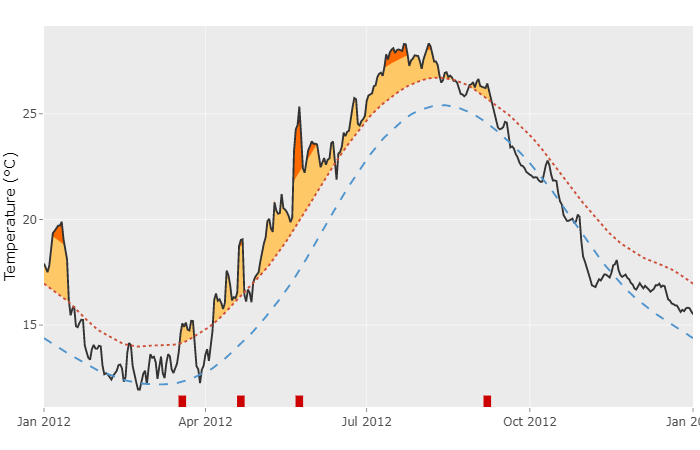
\includegraphics[width=0.75\textwidth, angle =0]{Chapter3/NorthWestAtlantic2012/NwAtlantic.png}
        }
            \caption{A figure of SST at 37$^{\circ}$N 287$^{\circ}$E where recorded temperatures are indicated by the black line, expected temperatures (climatology) is indicated by the blue dashed line and 90th percentile temperatures are indicated by the red dotted line. Hence, the filled colour area indicates MHW days, where the darker the shade, the higher the intensity of the MHW. \cite{MHWtracker}}
            \label{fig:NwAtlantic}
\end{figure}

\noindent Looking at \autoref{fig:NwAtlantic}, we can the MHW started just after April, 2012 and continued onto August 2012 lasting around 200 days in the region we are investigating, just east of Virginia, USA.
\\\\
To begin investigating the impacts this MHW had on the health of phytoplankton we can use our Chlorophyll concentration data for the same location and build a ARIMA model, we can then compare the raw data to our model to see if the MHW causes any anomalies.
\\\\
Looking at \autoref{fig:NwAtlanticTS}, we can see the recorded chlorophyll concentration is lower than the ARIMA model from the second month in. This could be due to the MHW period showed at the start of 2012 in \autoref{fig:NwAtlantic} where SST where as high as 20 Celsius. The raw data than continues to be below the model till around late September when there is a very sharp increase in chlorophyll concentration which goes considerable higher than what the model predicted and at a much faster rate. This sharp increase in chlorophyll concentration hints at a chlorophyll bloom. If we again refer to \autoref{fig:NwAtlantic}, we can see a the SST begins to fall around September which could be responsible for the chlorophyll bloom. To investigate further we will analyse the annual climatology of chlorophyll concentration.

\begin{figure}[H]
\centering
    \makebox[\textwidth][c]{
        \includegraphics[width=0.5\textwidth, angle =-90]{Chapter3/NorthWestAtlantic2012/Data_37N287E_Chl_TS.eps}
        }
            \caption{A figure of our ARIMA model calculated using our chlorophyll data set and our raw data for 37$^{\circ}$N 287$^{\circ}$E}
            \label{fig:NwAtlanticTS}
\end{figure}

Looking at \autoref{fig:NwAtlanticCl} we can see how the maximum chlorophyll concentration is often seen in the first six months, but during the year of our heatwave the peak came much later in the year. Despite the recorded SST following roughly the same shape as SST climatology plot indicted by the blue dashed line in \autoref{fig:NwAtlantic}. This further shows the anomalous behaviour. 

\begin{figure}[H]
\centering
    \makebox[\textwidth][c]{
        \includegraphics[width=0.5\textwidth, angle =-90]{Chapter3/NorthWestAtlantic2012/Data_37N287E_Chl_Climatology.eps}
        }
            \caption{Annual climatology for chlorophyll concentration at 37$^{\circ}$N 287$^{\circ}$E}
            \label{fig:NwAtlanticCl}
\end{figure}

\subsection{Mediterranean Sea (2003)}

During 2003 the Mediterranean Sea saw it's largest event recorded, being on average $4^{\circ}$C for 30 days, from this event saw mass mortality of marine life in the surrounding rocky reefs.

\begin{figure}[H]
\centering
    \textbf{-37$^{\circ}$N 287$^{\circ}$E}\par
    \makebox[\textwidth][c]{
        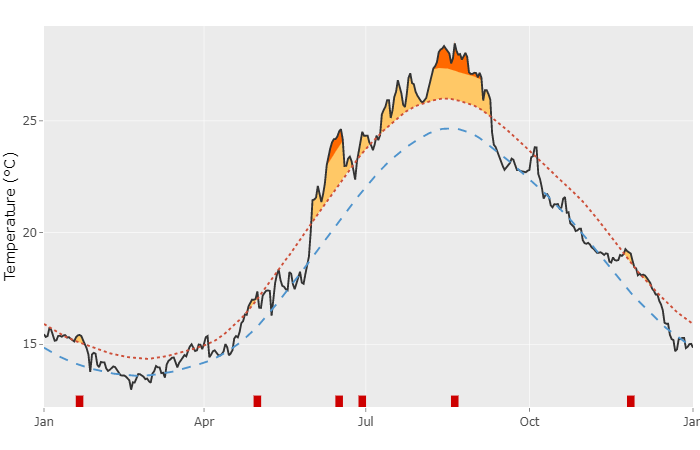
\includegraphics[width=0.75\textwidth, angle =0]{Chapter3/ArabianSea/MS.png}
        }
            \caption{A figure of SST at 40$^{\circ}$N 06$^{\circ}$E between January 2012 - January 2013. Recorded temperatures are indicated by the black line, expected temperatures (climatology) is indicated by the blue dashed line and 90th percentile temperatures are indicated by the red dotted line. Hence, the filled colour area indicates MHW days, where the darker the shade, the higher the intensity of the MHW. \cite{MHWtracker}}
            \label{fig:MS}
\end{figure}

Looking at figure \autoref{fig:MS}, we can see the MHW starts around the start of June and continues till around the middle of September.  
\\\\
Again to investigate the impacts this MWH may of had on the health of phytoplankton we will produce a ARIMA model using our chlorophyll concentration data and compare it to our recorded data and try to find any anomalies that may have been caused by the abnormally high SST.
\\\\
Looking at \autoref{fig:MSts}, we can see that the chlorophyll concentration is mostly lower than what would be expected from our ARIMA model. This is in accordance with what we would expect due to the lower availability of nutrients for the phytoplankton to consume in warm water.

\begin{figure}[H]
\centering
    \textbf{40$^{\circ}$N 06$^{\circ}$E}\par
    \makebox[\textwidth][c]{
        \includegraphics[width=0.5\textwidth, angle =-90]{Chapter3/ArabianSea/Data_40N6E_Chl_TS.eps}
        }
            \caption{A figure of our ARIMA model calculated using our chlorophyll data set and our raw data for 40$^{\circ}$N 06$^{\circ}$E}
            \label{fig:MSts}
\end{figure}

\section{Conclusion}

After establishing a casual relationship between SST and chlorophyll concentration using regression analysis. We then found published literature that justified the relationship using physical and biological systems that are known about the ocean and phytoplankton. We then extended this relationship into two well-documented MHWs, the 2012 North West Atlantic and 2003 Mediterranean Sea MHW, which back up the casual relationship. To improve upon our relationship, we could further our research into other variables that MHWs alter, other than SST. Such as ocean currents and investigate the impact that these other variables have on phytoplankton and mechanism they rely on. A deeper look into the exchange of nutrients between ocean layers would also deepen our understanding as we only considered it simple when in fact it is a very complex system which relies on many variables such as distance to the equator, the hemisphere you are on and atmospheric conditions, it could prove important to find which factor between location and temperature have the biggest impact on the health of phytoplankton. 

%\begin{figure}[H]
\centering
    \textbf{Sea Surface Temperature at 40N290E}\par
    \makebox[\textwidth][c]{
        \includegraphics[width=0.75\textwidth, angle =0]{Chapter3/NorthWestAtlantic2012/NwAtlantic2012.png}
        }
            \caption{A figure of SST at 40N290E where recorded temperatures are indicated by the black line, expected temperatures (climatology) is indicated by the blue dashed line and 90th percentile temperatures are indicated by the red dotted line. Hence, the colour area indicates MHW days, where the darker the shade the higher the intensity. \cite{MHWtracker}}
            \label{fig:}
\end{figure}

\bibliographystyle{alpha}
\bibliography{mybibliography.bib}

\end{document}